The statistical modelling of human behaviour is a difficult task \cite{human_behaviour}. Human event data arise in a variety of real-world situations, for example when inspecting network traffic or email communications, and being able to find anomalies has important applications in botnet detection and spotting suspicious behaviour on social networks. In this project, we attempted to model the behaviour of one user of Twitter using various random processes. Ideally, we would find a good model for Twitter in general, but one user makes a worthy starting point, and Twitter provides an easily accessible representation of such data without trawling through network logs or other people's email accounts. The user was observed over the course of around 6 months posting (emitting) a little over 3,300 tweets. The goal is to find some kind of model to fit these data, without using a hideously large number of parameters.

The data are visualised in Figure \ref{raw_data}. We see a little seasonality - the user seems to be going to sleep at some time, waking up at another time, as well as some ``burstiness" where the user produced a very rapid series of tweets in a very short time. Being able to detect these features would let us intuitively decide whether a fit is good or not, but principally we'll be reliant on statistical tests to judge how good our model is.

Chapter \ref{zoo} will define a series of stochastic processes which we can use for modelling the data, and then chapter \ref{techniques} will apply the more relevant ones. Of particular note is the Markov-Modulated Poisson Process defined in \textsection\ref{mmppdef}, which several authors \cite{mmpp1}\cite{mmpp2}\cite{mmpp3} have postulated will provide a good model due to its doubly-stochastic nature -- the intuition being that the tweets are a stochastic process, and the parameters of that stochastic process themselves follow another stochastic process. We will attempt to fit this and a series of other models, before concluding that a Discrete Time Hidden Markov Model with lognormal emissions provides the best fit.

Appendix \ref{fun} also describes a minor result which was spotted during this project, and which may have rather useful applications in other fields.

\begin{figure}[h]
\centering
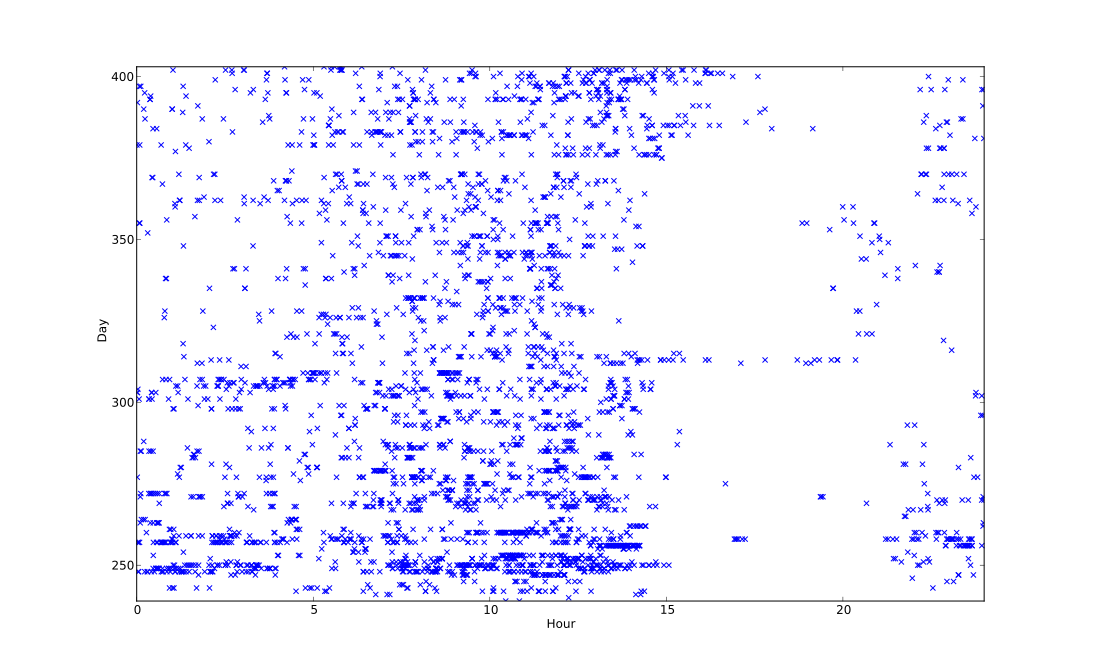
\includegraphics[width = 0.5\textwidth]{./images/raw_data.png}
\caption{The raw data gathered from the Twitter user. Each blue cross marks a tweet at a particular time. The 24 hours of a day run across the x axis, and the days within our 6 months run up the y-axis, so a point at $(17.5, 256)$ is a tweet at 5:30pm 256 days into the observation.}
\label{raw_data}
\end{figure}